\documentclass[11pt]{article}
\usepackage[utf8]{inputenc}
\usepackage{geometry}
\usepackage{booktabs}
\usepackage{graphicx}
\usepackage{hyperref}
\usepackage{amsmath}
\usepackage{amssymb}
\usepackage{caption}

\title{Preferences in AI Project Report}
\author{Pratik Deshmukh}
\date{\today}

\begin{document}

\maketitle

\section{Introduction}
This report presents experiments on free-riding in sequential decision-making
under different \emph{statistical cultures}, following the framework of
\cite{lackner2023freeriding}. Our goal is to replicate the structure of Section~5
of that work while extending it with additional statistical cultures.

\section{Background}

\subsection{Multi-Issue Model}
We study sequential decision-making in \emph{multi-issue elections}, where a set
of voters must decide on several issues, each with multiple candidates. Each
voter submits approval preferences for all candidates on each issue. A voting
rule is then applied issue by issue to determine the collective outcome.

\subsection{Voting Rules}
We focus on two families of rules, as in \cite{lackner2023freeriding}:

\begin{itemize}
    \item \textbf{Sequential Utilitarian Rule:} selects in each issue the
    candidate with the highest total number of approvals. This rule is equivalent
    to the \emph{mean OWA} and is immune to manipulation.
    \item \textbf{Thiele-Based Rules:} a general class where voter satisfaction
    decreases marginally as more of their approved candidates are selected.
    We evaluate sequential Thiele rules with parameters $x \in \{1,5,7\}$,
    where the case $x=0$ corresponds to utilitarian aggregation.
    \item \textbf{OWA-Based Rules:} aggregate voter satisfaction using Ordered
    Weighted Averages (OWAs). We evaluate parametric OWA rules with
    $x \in \{1,5,10,15\}$, interpolating between utilitarian ($x=0$) and
    leximin ($x=n-1$). For completeness, we also include the explicit
    \emph{leximin OWA}.
\end{itemize}

\subsection{Statistical Cultures}
The way preferences are generated strongly influences manipulation risks.
We consider four cultures:
\begin{itemize}
    \item \textbf{p-IC}: per-issue impartial culture, sampling approvals
    independently with probability $p$.
    \item \textbf{Disjoint Groups}: voters are divided into $g$ groups with
    internally aligned preferences.
    \item \textbf{Resampling Model}: preferences are generated by resampling
    with parameters $(p, \phi)$ controlling randomness and correlation.
    \item \textbf{Hamming Noise}: preferences are first generated from another
    culture and then perturbed by flipping approvals with small probability.
    This noise model is slightly different from that used in
    \cite{lackner2023freeriding}, but serves the same purpose of modeling
    robustness under perturbations.
\end{itemize}

\subsection{Risk Metrics}
We evaluate manipulation opportunities using the following metrics:
\begin{itemize}
    \item \textbf{Trials:} total number of manipulation attempts.  
    \item \textbf{Successes:} number of manipulations that improved the manipulator’s outcome.  
    \item \textbf{Harms:} number of manipulations that backfired on the manipulator.  
    \item \textbf{Success rate:} proportion of trials with a successful manipulation.  
    \item \textbf{Harm rate:} proportion of trials with a harmful manipulation.  
    \item \textbf{Risk:} ratio of harms to successes.  
\end{itemize}

\section{Methodology}
We repeat the experiments from Section~5 of \cite{lackner2023freeriding},
using four statistical cultures: impartial culture (p-IC), disjoint groups,
the $(p, \phi)$-resampling model, and the Hamming-noise model. For each, we run
multiple seeds and compare risk metrics under sequential utilitarian,
sequential Thiele rules ($x=1,5,7$), and OWA rules ($x=1,5,10,15$, plus leximin).

\subsection{Parameters}
For transparency, we explicitly document the parameters used in our experiments:

\begin{itemize}
    \item \textbf{p-IC}: approval probability $p=0.5$.
    \item \textbf{Disjoint}: voters are partitioned into $g = 2$ groups with
    aligned preferences.
    \item \textbf{Resampling}: parameters $(p,\phi) = (0.5,0.5)$, consistent
    with the disjoint model.
    \item \textbf{Hamming noise}: perturbations introduced by flipping a
    voter’s approval with probability $0.1$ per issue.
\end{itemize}

For all cultures, we fix the number of voters $n=20$, issues $k=5$, and
$c=4$ candidates per issue. Each configuration is run with 30 random seeds.

\section{Results}
The combined results table is automatically generated by the experiment
pipeline. The table below is included directly from the output file:

\begin{table}[h!]
\centering
\resizebox{\textwidth}{!}{%
\input{tables/combined.tex}
}
\caption{Combined results across cultures and rules. Risk metrics include trials,
successes, harms, success and harm rates, and risk (harms/successes).}
\label{tab:combined}
\end{table}

\subsection{Per-Culture Comparisons}

\paragraph{p-IC.}
\begin{figure}[h!]
\centering
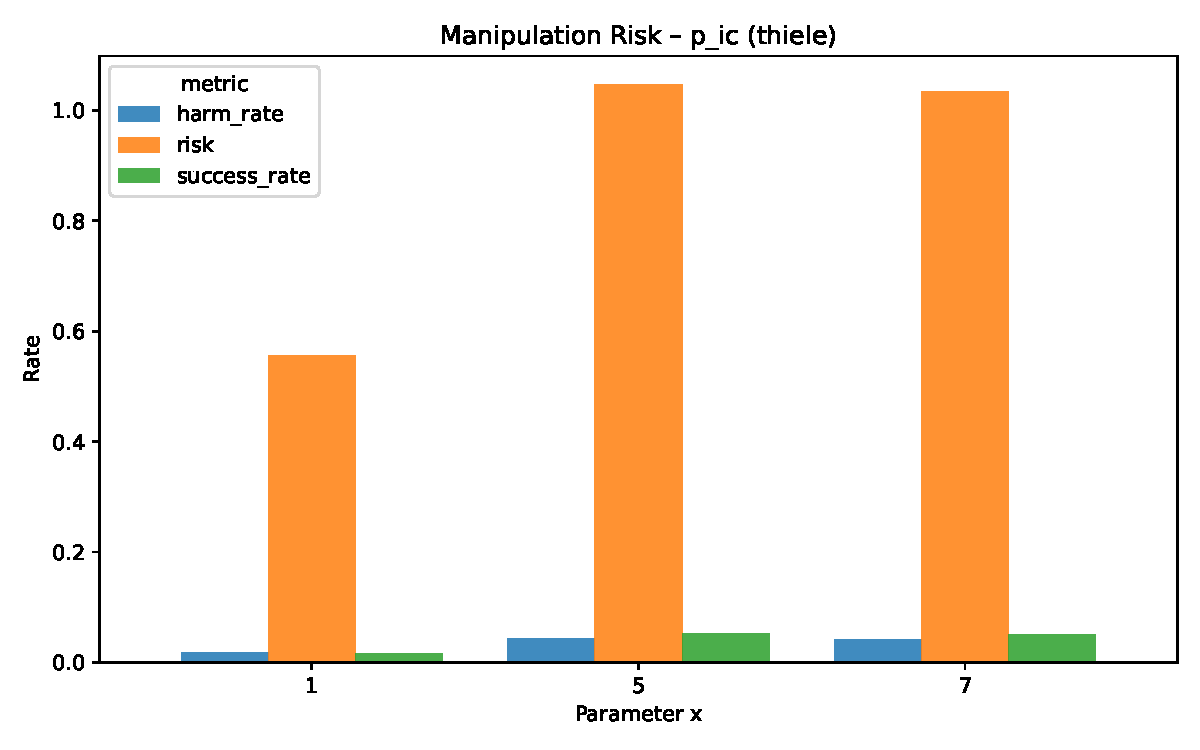
\includegraphics[width=0.7\textwidth]{figures/risk_p_ic_thiele.pdf}
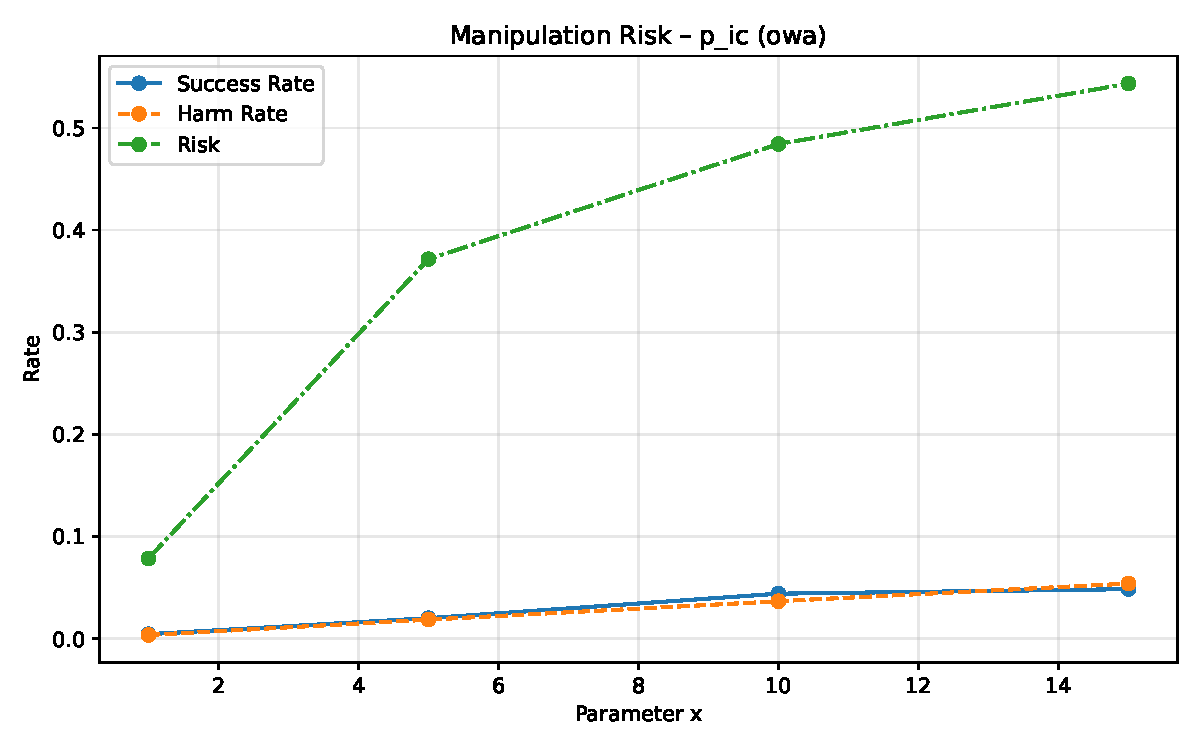
\includegraphics[width=0.7\textwidth]{figures/risk_p_ic_owa.pdf}
\caption{Manipulation risk under p-IC culture. Top: Thiele rules. Bottom: OWA rules.}
\end{figure}

\paragraph{Disjoint Groups.}
\begin{figure}[h!]
\centering
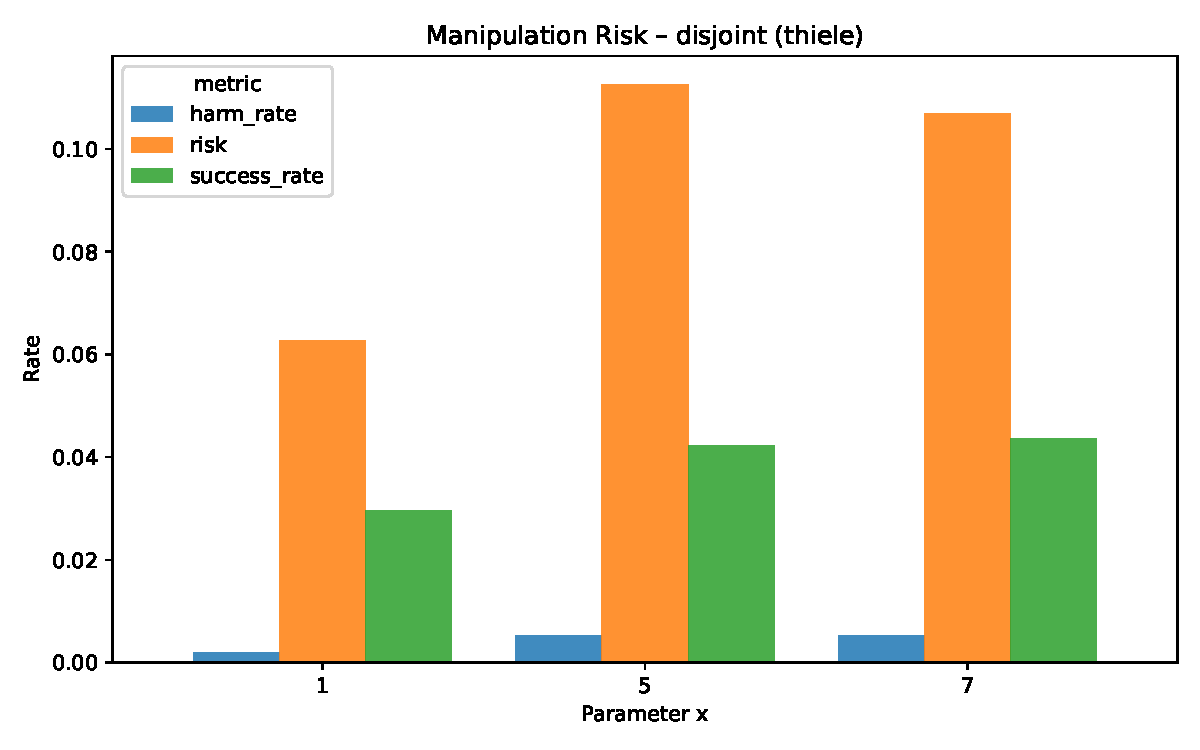
\includegraphics[width=0.7\textwidth]{figures/risk_disjoint_thiele.pdf}
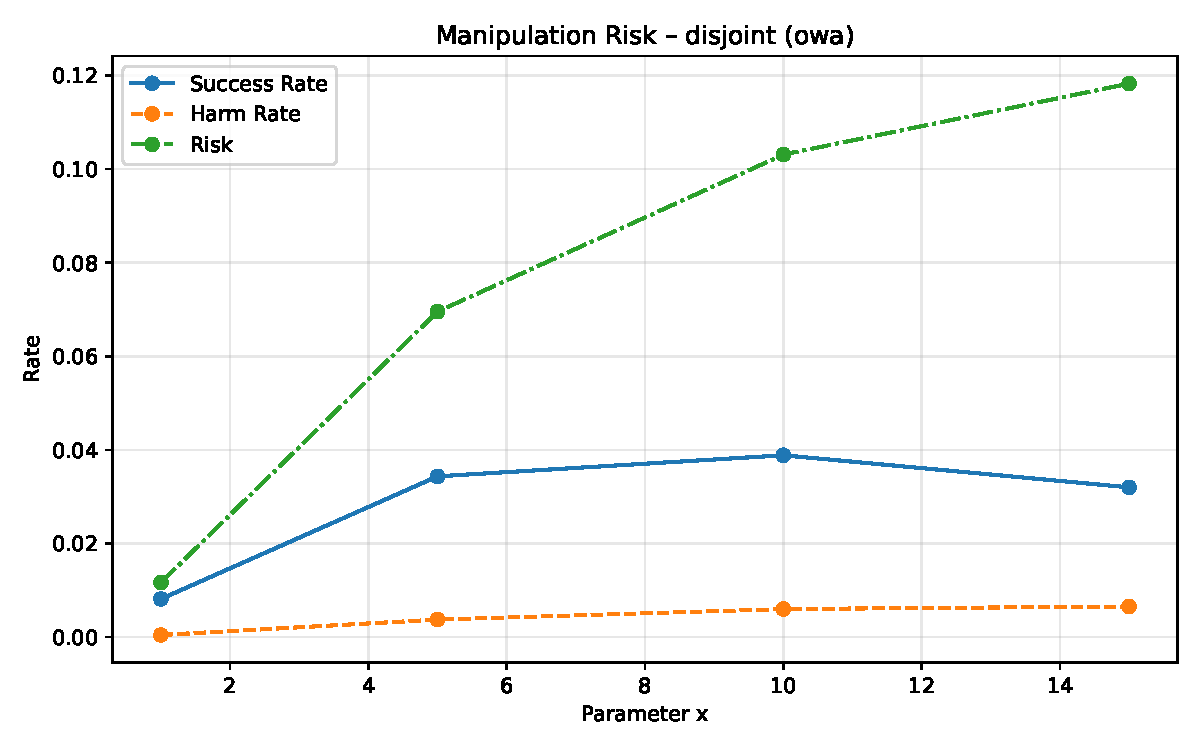
\includegraphics[width=0.7\textwidth]{figures/risk_disjoint_owa.pdf}
\caption{Manipulation risk under disjoint-group culture. Top: Thiele rules. Bottom: OWA rules.}
\end{figure}

\paragraph{Resampling Model.}
\begin{figure}[h!]
\centering
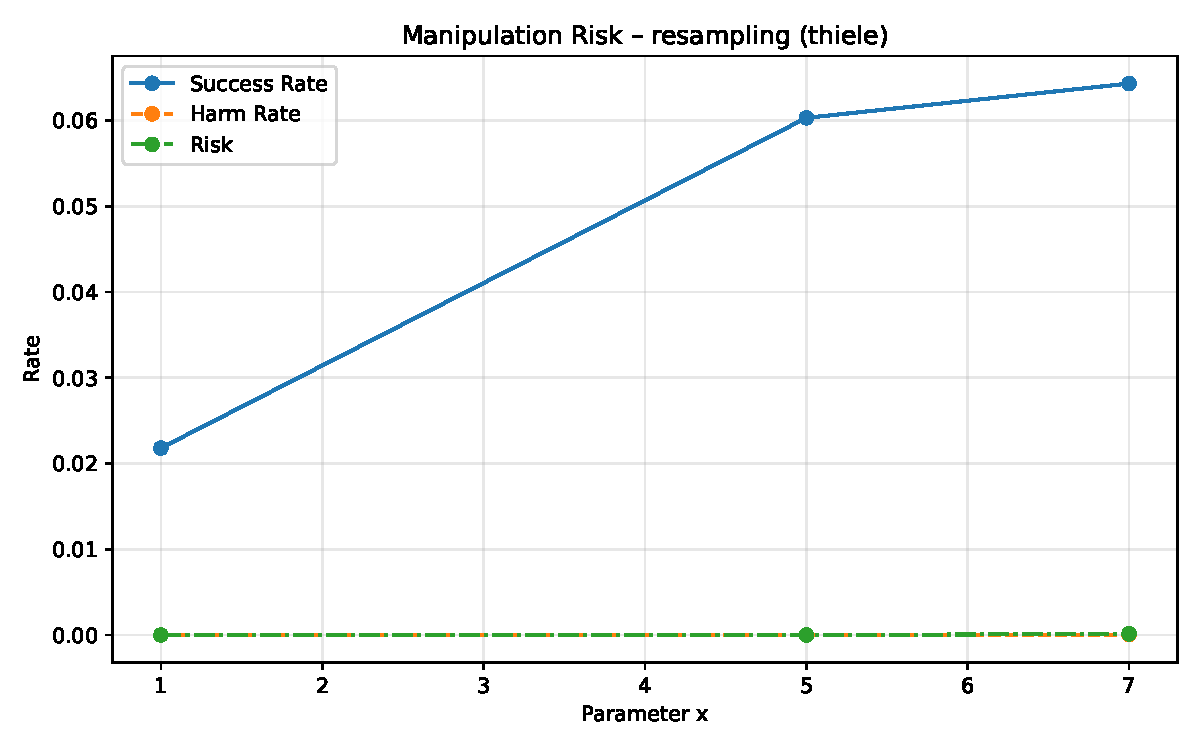
\includegraphics[width=0.7\textwidth]{figures/risk_resampling_thiele.pdf}
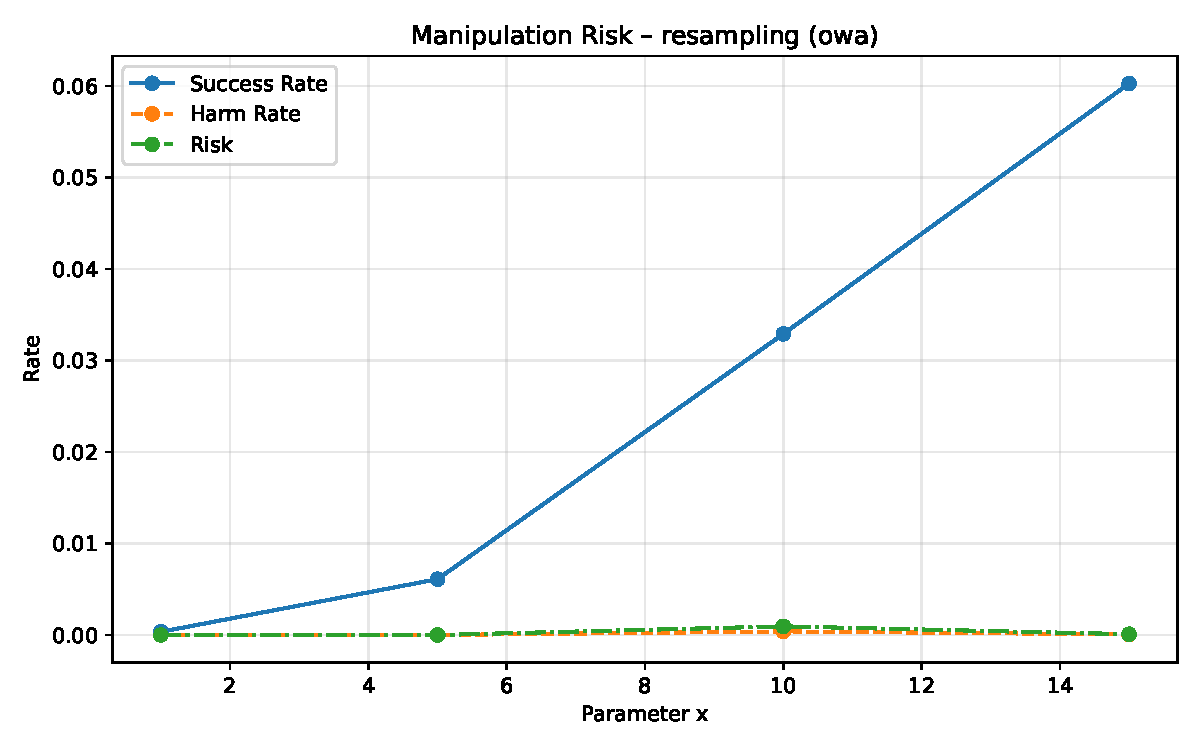
\includegraphics[width=0.7\textwidth]{figures/risk_resampling_owa.pdf}
\caption{Manipulation risk under resampling culture. Top: Thiele rules. Bottom: OWA rules.}
\end{figure}

\paragraph{Hamming Noise.}
\begin{figure}[h!]
\centering
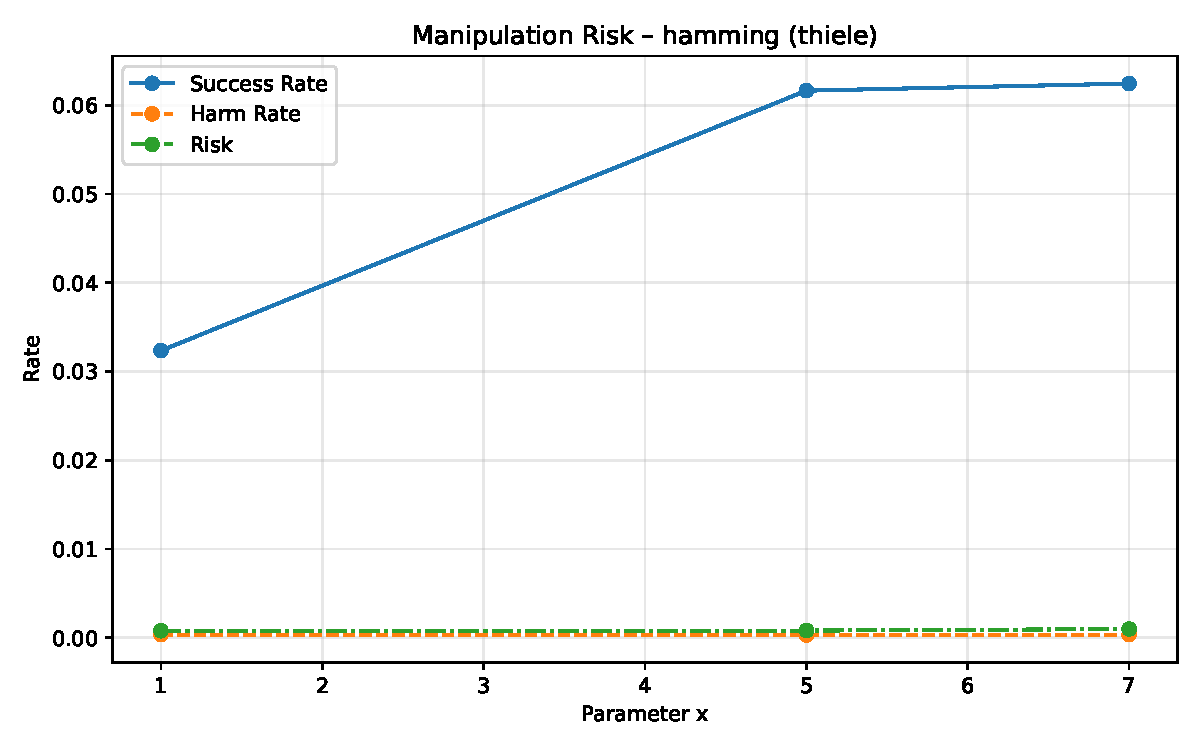
\includegraphics[width=0.7\textwidth]{figures/risk_hamming_thiele.pdf}
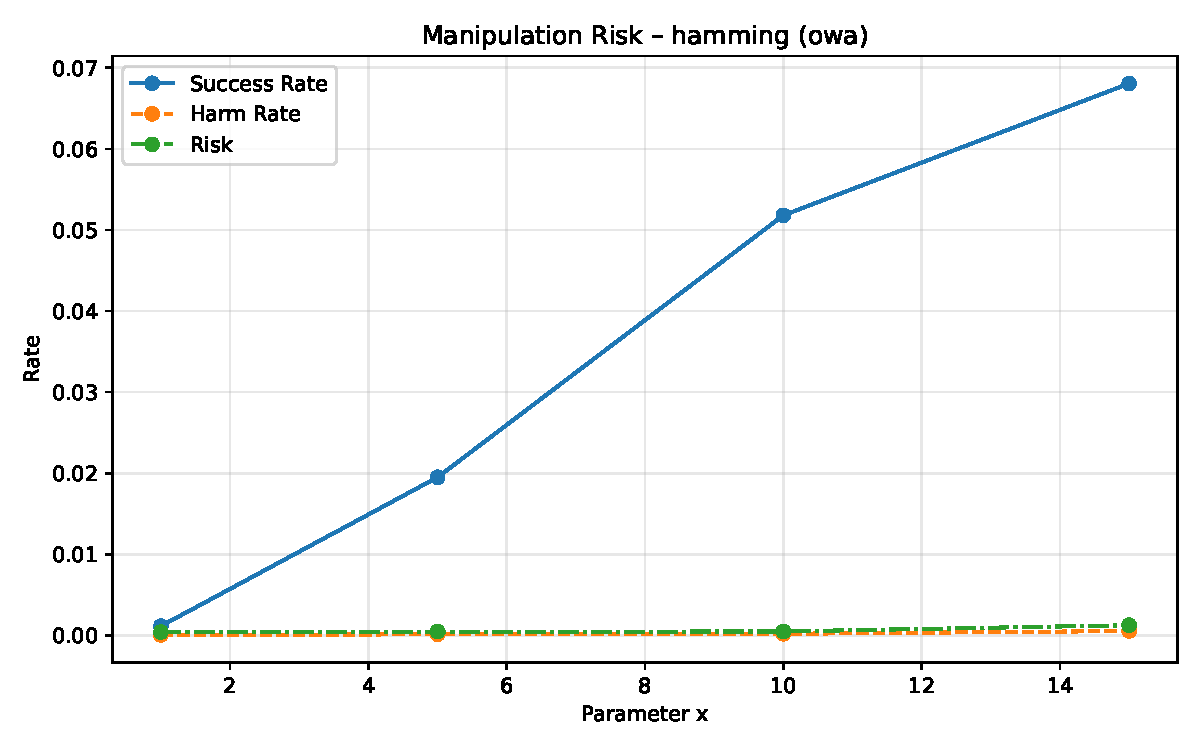
\includegraphics[width=0.7\textwidth]{figures/risk_hamming_owa.pdf}
\caption{Manipulation risk under Hamming-noise culture. Top: Thiele rules. Bottom: OWA rules.}
\end{figure}

\section{Discussion}
Our experiments highlight the dependence of manipulation risk on both the
voting rule and the statistical culture.

\paragraph{Effect of Statistical Cultures.}
The \emph{p-IC} culture exhibits moderate manipulation opportunities.
The \emph{disjoint} model produces clearer group structures, sometimes
increasing manipulation success rates. The \emph{resampling} model yields
non-negligible risks depending on $\phi$, and the \emph{Hamming noise}
experiments show that random perturbations can both increase and decrease
manipulation opportunities, depending on the rule.

\paragraph{Effect of Voting Rules.}
The \emph{utilitarian rule} (equivalently mean OWA) is immune to manipulation.
Thiele rules with larger $x$ increase proportionality but are more exposed to
free-riding opportunities. OWA rules interpolate between utilitarian and
leximin: intermediate parameters show manipulation risks, while leximin tends
to reduce success rates but sometimes increases harms.

\paragraph{Risk Metrics.}
Across all settings, harm rates are non-negligible, confirming that attempts at
manipulation carry real risks. In particular, when manipulation succeeds, it is
often accompanied by harmful attempts that worsen outcomes for manipulators.

\section{Conclusion}
Our experiments confirm that the choice of statistical culture strongly
influences manipulation risks. Cultures with correlated preferences (e.g.,
disjoint, resampling) can increase opportunities for manipulation, while random
noise can unpredictably alter them. 

Across voting rules, utilitarian aggregation is immune. Thiele-based rules and
OWA-based rules illustrate trade-offs: increasing proportionality or fairness
typically comes at the expense of higher manipulation risk.

Future work should extend these experiments by exploring richer grids of
parameters $(p,\phi)$, noise rates, and group structures. Replicating the
visualization style of \cite{lackner2023freeriding} with further plots would
also allow direct side-by-side comparison of manipulation risks across rules.

\section*{Repository}
The full project code and report sources are available at: \\
\href{https://github.com/inquisitour/preferences-in-ai}{github.com/inquisitour/preferences-in-ai}

\bibliographystyle{plain}
\bibliography{references}

\end{document}
% !TEX root = report.tex
